\section{Example Scenario}\label{s:deploy}
\begin{figure*}[t]
    \centering
    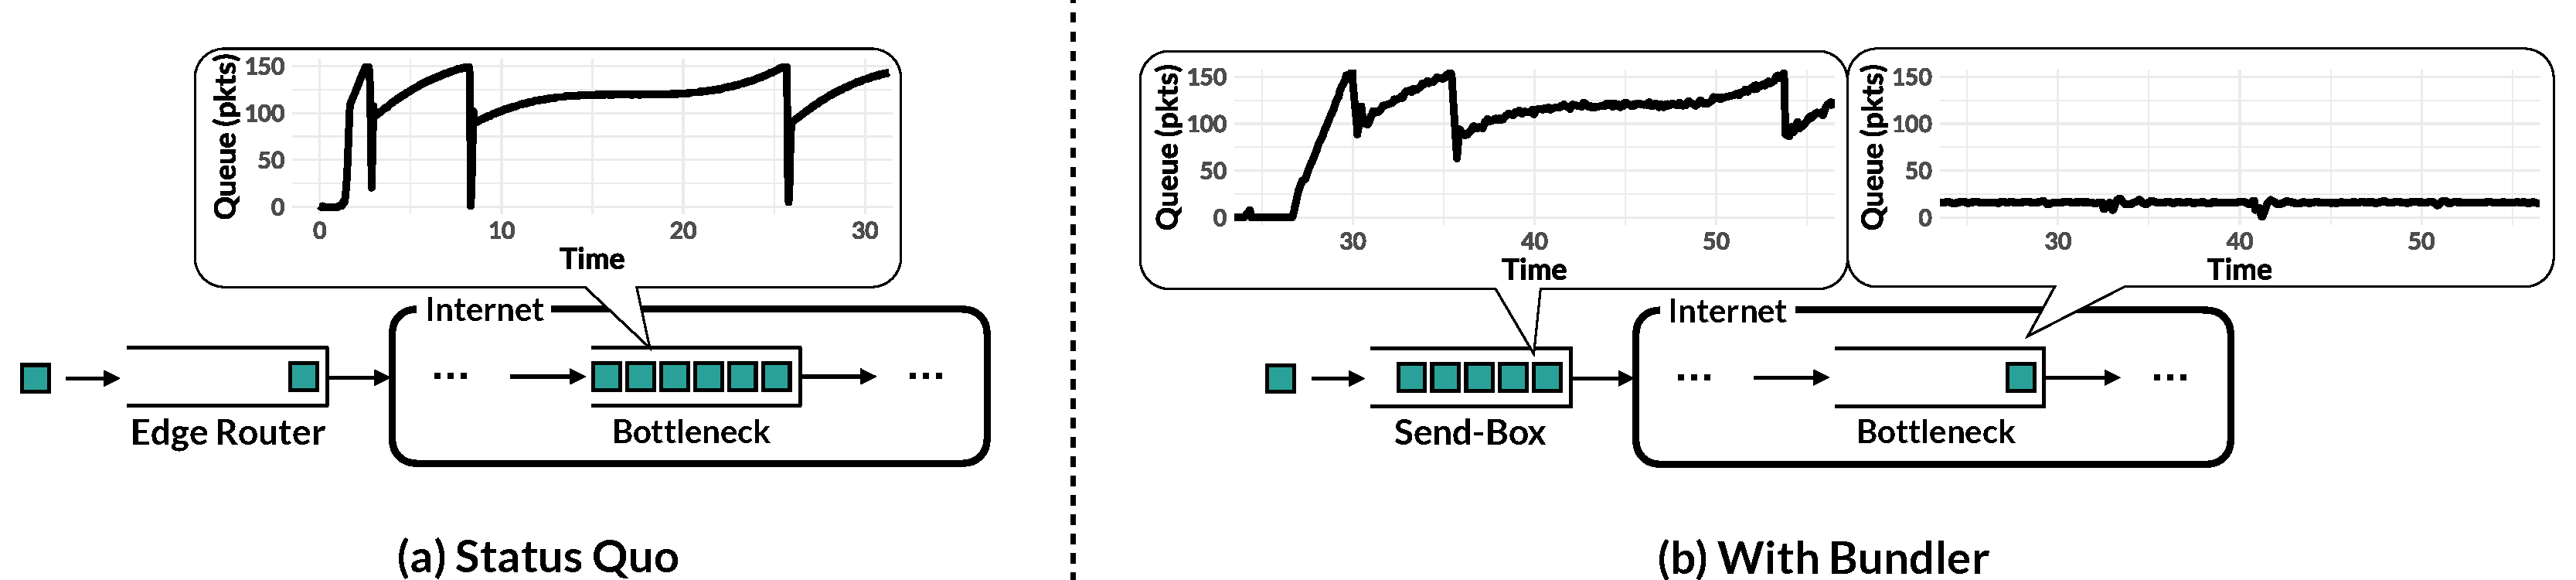
\includegraphics[width=\textwidth]{img/shift-bottleneck-combined}
    \caption{This illustrative example with a single flow shows how \name can take control of queues in the network. The plots, from measurements on and emulated path (as in \S\ref{s:eval}), show the trend in queueing delays at each queue over time. The queue where delays build up is best for scheduling decisions, since it has the most choice between packets to send next. Therefore, the \inbox \emph{shifts} the queues to itself to gain scheduling power.}\label{fig:design:shift-bottleneck}
\end{figure*}
%

\fc{Would it be better to lead with some example of how theres a large amount
of traffic bewteen A and B? }

Figure~\ref{fig:deploy:arch} provides an example scenario for deploying \name. 
\name aggregates traffic from Domain A to Domain B, and vice-versa, into two unidirectional bundles. 
Then, on egress, the \inbox moves the in-network queues built by the bundled traffic to itself (we describe the specific mechanism in \S\ref{s:design}). 
It can thus enforce desired scheduling policies across the traffic in the bundle.
The performance benefits that this provides are dictated by the following.

\Para{Amount of Aggregation} 
A traffic bundle, to be useful, must be \emph{heavyweight} enough to drive self-inflicted queueing in the network; these queues, once under \name's control, provide scheduling opportunities. We expect many bundles to be heavyweight in practice because a majority of Internet traffic today is owned by a few large content providers who host a wide array of services~\cite{fivecomps, labovitz}. 
In our example scenario, the bundles between Domain A and B might comprise large amounts of traffic generated by various services (such as email, messaging, video streaming, cloud storage etc.) hosted by the content provider and used by different clients within the enterprise. 
%\radhika{The bundle from domain B to A would similarly be heavyweight, though possibly lighter than the bundle in the opposite direction.}
%\an{maybe good to list examples of what this would consist of, in case people just think of ACKs. Maybe backups? But several of the applications above (\eg video) are already bi-directional.}
%Furthermore, it is possible to observe self-inflicted queueing even by sending from a single machine; we take advantage of this in experiments on real Internet paths in \S\ref{s:eval}. \radhika{chop last line?}

\Para{Congestion in the middle of the network} 
Content providers already have control over packets which queue within their own domains~\cite{swan, b4, bwe}. \name is useful for moving queues that build up due to congestion in the middle of the network (\ie between a \pair).
The next question that arises is, does such in-network congestion occur in practice? A recent measurement study~\cite{inferring-interdomain-congestion} indicates that inter-domain links in the network (such as the red bottleneck link in Figure~\ref{fig:deploy:arch}) can indeed experience significant congestion. 
We briefly discuss how the nature of this congestion influences \name's benefits (and provide detailed results in \S\ref{s:eval}).

\paragraphi{Self-inflicted congestion} This occurs when traffic from a single bundle causes a queue to build up at the bottleneck links in the network, even without any other cross-traffic. It can happen when a small carrier network does not have enough capacity to sustain the large volume of traffic sent by a content provider to a receiving domain, or due to explicit rate limiting commonly done by ISPs~\cite{isp-throttle-1, isp-throttle-2, isp-throttle-3}. In such cases, \name can result in
significant improvements in performance \an{up to XX\%}, as it would then have control over the entire queue. 
%In our experiments (\S\ref{s:eval}), we found this to be the case.

\paragraphi{Congestion due to bundled cross-traffic} In-network congestion can further increase in the presence of other cross-traffic (\eg when the peering link between Carrier B and the enterprise in Figure~\ref{fig:deploy:arch} is shared by traffic from multiple content providers' domains). 
\name continues to provide benefits (\an{up to YY\%}) when the competing flows are part of other bundles from/to other domains because the rate control algorithm at each of the other {\inbox}es would ensure that the in-network queues remain small. Since each \inbox controls its own delays, it can apply the appropriate scheduling policy in its the per-bundle queues.
We expect this to become the common form of observed congestion as more domains deploy \name. 

\paragraphi{Congestion due to un-bundled cross-traffic} We now consider the scenario where the cross-traffic includes flows from domains that have not yet deployed a \name. If all such \emph{un-bundled} competing flows are short-lived (up to a few MBs), the bundled traffic still sees significant performance benefits (\an{ZZ \%}). 
However, if the cross traffic is long lasting and aggressively fills up available buffer space at the bottleneck link, using a delay-based congestion controller  at the \name would adversely impact the bundled traffic. Instead, \name detects the presence of such \emph{buffer-filling} cross-traffic and, to compete fairly, pushes more packets into the network (as described in \S\ref{s:queue-ctl}). It thus relinquishes its control over the bundled traffic, and falls back to the status-quo performance.
%This scenario is a limitation of \name's design, since it forces \name to fall back to status-quo performance.
%\an{reword} 
Such buffer-filling flows are unlikely to arrive very frequently~\cite{caida-dataset}. 

\vspace{0.05in}
\paragrapha{Takeaway} While \name must revert to status quo performance in the face of aggressive, buffer-filling cross traffic, in most scenarios it significantly improves performance (as we will show in \S\ref{s:eval}).
This, combined with its deployment ease, makes a strong case for deploying \name. 
